\documentclass[aspectratio=169]{wzbeamer}
\usepackage[hyperref=true,style=numeric,backend=biber,sorting=nty,autocite=inline,backref=true,urldate=iso,date=iso,seconds=true]{biblatex}
\addbibresource{ref.bib}
\usepackage{animate}
\usetheme[progressbar=frametitle, numbering=counter]{metropolis}
\usepackage{fontspec}
\setmainfont{Times New Roman}
\setsansfont{Arial}
\setmonofont{Cambria}

\usepackage{etoolbox} % for '\AtBeginEnvironment' macro
\AtBeginEnvironment{pmatrix}{\everymath{\displaystyle}}

\graphicspath{{./figs/}}

\title{Liouville's Theorem and Jarzynski Equality}
\subtitle{平统讨论班}
\author{王准}
\institute[pku]{北京大学}

\setbeamertemplate{section in toc}[circle]
\setbeamertemplate{subsection in toc}[ball unnumbered]
\begin{document}
\maketitle 
    
\begin{frame}{Overview}
    \begin{multicols}{2}
		\tableofcontents
    \end{multicols}
\end{frame}


\section{Liouville Theorem}
    \subsection{Proof}
    \begin{frame}{Liouville定理}
        \begin{alertblock}{Liouville定理}
            系统按照满足哈密顿正则方程演化时, 微观态密度分布沿系统轨迹保持为常数, 即,
            \begin{equation}
                \dv{\rho}{t} = 0
            \end{equation}
        \end{alertblock}

    \end{frame}
    \begin{frame}{证明1}
        哈密顿量$H = H(\vb*q, \vb*p) = H(\vb*x)$, $\vb*x = (\vb*q, \vb*p)$
        \begin{equation}
            \left\{
            \begin{split}
                \dot{q}_i &= \pdv{H}{p_i}\\
                \dot{p}_i &= - \pdv{H}{q_i}
            \end{split}
            \right.\quad
            \Rightarrow\quad
            \dot{x}_\alpha = \omega_{\alpha\beta} \pdv{H}{x_\beta}
        \end{equation}
        其中, $i = 1,2,\dots,n, \ \alpha = 1,2,\dots,2n$, 
        \begin{equation}
            [\omega_{\alpha\beta}] = 
            \begin{pmatrix}
                & I \\
                -I & 
            \end{pmatrix}
            \quad\Rightarrow\quad
            \omega_{\alpha\beta} = -\omega_{\beta\alpha}
        \end{equation}
    \end{frame}
    
    \begin{frame}{证明1}
        相空间中, 微观态的数量应该保持不变, 可以写出流和密度满足的守恒关系,
        \begin{equation}
            \pdv{\rho(\vb*x, t)}{t} + \pdv{x_\alpha}(\dot x_\alpha \rho(\vb*x,t) ) = 0
        \end{equation}
        从而,
        \begin{equation}
            \begin{split}
                \dv{\rho(\vb*x(t),t)}{t} =& \pdv{\rho}{t} + \dot x_\alpha \pdv{\rho}{x_\alpha}\\
                =& - \rho\cdot \pdv{x_\alpha}\dot x_\alpha\\
                =& - \rho\cdot \omega_{\alpha\beta} \pdv{H}{x_\alpha}{x_\beta}\\
                =& \ 0
            \end{split}
        \end{equation}
    \end{frame}
    \begin{frame}{证明2}
        从演化的角度考虑, 微观态数目不变可以表述为,
        \begin{equation}
            \rho(\vb*x_t,t) \dd\vb*x_t = \rho(\vb*x_0,0) \dd\vb*x_0, \quad\vb*x_t = \vb*x(t)
        \end{equation}
        其中, $\dd\vb*x_t$表示体积元. 我们如果将时间演化视作一种变换, 
        \begin{equation}
            \phi_{s\to t} : \vb*x_s \mapsto \vb*x_t,\quad \text{i.e.}\ \vb*x_t = \phi_{s\to t} (\vb*x_s)
        \end{equation}
        那体积元之间的关系就应该由Jacobi行列式决定,
        \begin{equation}
            \dd\vb*x_t = \det(\pdv{\vb*x_t}{\vb*x_0}) \dd\vb*x_0 = J(t) \dd\vb*x_0
        \end{equation}
    \end{frame}
    \begin{frame}{证明2}
        求$J(t)$对时间的导数,
        \begin{equation}
            \begin{split}
                \dv{J}{t} &= \sum_\alpha \det(\pdv{(\dots ,\dot x_{t, \alpha}, \dots)}{\vb*x_0})\\
                &= \sum_\alpha \det(\pdv{(\dots ,\dot x_{t,\alpha}, \dots)}{\vb*x_t}) \cdot J(t)\\
                &= \sum_\alpha \pdv{\dot x_{t, \alpha}}{x_{t,\alpha}}\cdot J\\
                &= \omega_{\alpha\beta} \pdv{H}{x_{t,\alpha}}{x_{t,\beta}}\cdot J\\
                &= \ 0
            \end{split}
        \end{equation}
        $$ J \equiv 1 \quad \Rightarrow\quad \rho(\vb*x_t, t) = \rho(\vb*x_0, 0)$$ 
    \end{frame}
    \begin{frame}{Jacobi矩阵}
        Jacobi矩阵实际上就是向量函数对于向量自变量的导数, 
        \begin{equation}
            \pdv{\vb*y}{\vb*x} = [\pdv{y_i}{x_j}] = 
            \begin{pmatrix}
                \pdv{y_1}{x_1} & \pdv{y_1}{x_2} & \cdots & \pdv{y_1}{x_n}\\
                \pdv{y_2}{x_1} & \pdv{y_2}{x_2} & \cdots & \pdv{y_2}{x_n}\\
                \vdots & \vdots & & \vdots\\
                \pdv{y_n}{x_1} & \pdv{y_n}{x_2} & \cdots & \pdv{y_n}{x_n}
            \end{pmatrix}
        \end{equation}
        求导的链式法则也可以扩展到这个情形,
        \begin{equation}
            \pdv{\vb*z}{\vb*x} = \pdv{\vb*z}{\vb*y} \cdot \pdv{\vb*y}{\vb*x}
        \end{equation}
    \end{frame}
    \begin{frame}{证明2}
        证明2实际上给了一种新的观点, $\phi$是一个保持体积元大小不变的映射, 那么$\phi$就应该保持体积不变. 设$m$是相空间的Lebesgue测度(实际上就是体积), 对于可测集$A$,
        \begin{gather}
            m(A) = \int_A \dd \vb*x\\
            m(\phi(A)) = m(A)
        \end{gather}
        利用这一点, 我们可以将Poincar\'e定理运用到时间演化上.
    \end{frame}
    \subsection{Poincar\'e Reccurence Theorem}
    \begin{frame}{Poincar\'e定理}
        \begin{alertblock}{Poincar\'e定理(数学表述)}
            对于有限测度空间$(X,\Sigma,\mu)$, 若$f$是一个保测度的映射, 那么, $\forall E\in\Sigma$, 
            \begin{equation}
                \mu(\{x\in E: \exists N, \forall n > N, f^{\ n}(x) \notin E \}) = 0
            \end{equation} 
            即, 几乎所有的点都会在有限步回到$E$中.
        \end{alertblock}
    \end{frame}
    \begin{frame}{证明思路}
        令 $A_n = \bigcup_{k=n}^{\infty} f^{-k}E$, 表示了$E$中的点在$n$步以前的位置, 显然$E\subset A_0,\ \mu(A_n) = \mu(A_m)$, 
        \begin{equation}
            \mu(E - A_n) \leqslant \mu(A_0 - A_n) = \mu(A_0) - \mu(A_n) = 0
        \end{equation}
        而$\mu(E - \bigcap_{n=1}^\infty A_n) = \mu(\bigcup_{n=1}^\infty (E - A_n)) = 0 $, 表示了在所有在有限步没有回到$E$中的点.
    \end{frame}
    \begin{frame}{微正则系综中构造有限测度}
        微正则系综处于一个能壳$E\sim E+\dd E$上, 取$\dd n$为法向的线元, 我们有
        \begin{equation}
            |\nabla E|\dd n = \dd E  
        \end{equation}
        而我们知道时间演化是保持体积元的, 即$\dd S\dd n == \dfrac{\dd S}{|\nabla E|} \dd E$在时间演化下不变, 那么构造测度$\mu$,
        \begin{equation}
            \mu(A) = \int_A \frac{\dd S}{|\nabla E|}
        \end{equation}
        由于能壳总面积有限, 这是一个有限测度, 所以可以应用Poincar\'e定理. 即, 一个集合内的态几乎总会在有限时间的演化后回到初始的集合内.
    \end{frame}
    \begin{frame}{Poincar\'e定理和各态历经}
        统计物理中一个很重要的假设是各态历经, 它和Poincar\'e定理非常相似.
        \begin{itemize}
            \item 各态历经, 任意一个非零测度的集合$E$, 全空间$X$中最终不会到达$E$的点的测度为零.
            \item Poincar\'e, 任意一个非零测度的集合$E$, 从$E$出发最终不会到达$E$的点的测度为零.
        \end{itemize}
    \end{frame}
    % \documentclass[aspectratio=169]{wzbeamer}
% \usepackage[hyperref=true,style=numeric,backend=biber,sorting=nty,autocite=inline,backref=true,urldate=iso,date=iso,seconds=true]{biblatex}
% \addbibresource{ref.bib}
% \usepackage{animate}
% \usetheme[progressbar=frametitle, numbering=counter]{metropolis}
% \usepackage{fontspec}
% \setmainfont{Times New Roman}
% \setsansfont{Arial}
% \setmonofont{Cambria}

% \usepackage{etoolbox} % for '\AtBeginEnvironment' macro
% \AtBeginEnvironment{pmatrix}{\everymath{\displaystyle}}

% \graphicspath{{./figs/}}

% % \newcommand{\Pr}{\text{Pr}}
% \begin{document}
%++++++++++++++++++++++++++++++++++++++++++++++++++++++++++++++++++++++++++++++++++++++++++++++++++++++++++++++++++++++++++++++++++++++++++++++++++++++++++++++++++++++++++++++++++++++++++++++++++++++++++++++++++++++++++++++++++++++++++++++++++++++++++
\section{Jarzynski Equality}
    %==========================================================
    \subsection{Introduction}
    \begin{frame}{Jarzynski \& Crooks}
        \hspace{.05\textwidth}
        \begin{figure}
            \centering
            \subfigure[Christopher Jarzynski]{
                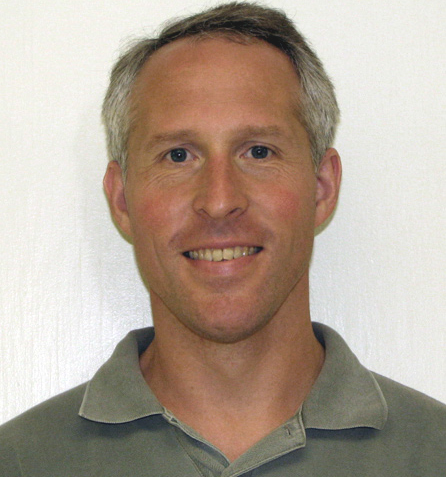
\includegraphics[width=.3\textwidth]{jarz.jpg}
            }
            \vspace{.05\textwidth}
            \subfigure[Gavin E. Crooks]{
                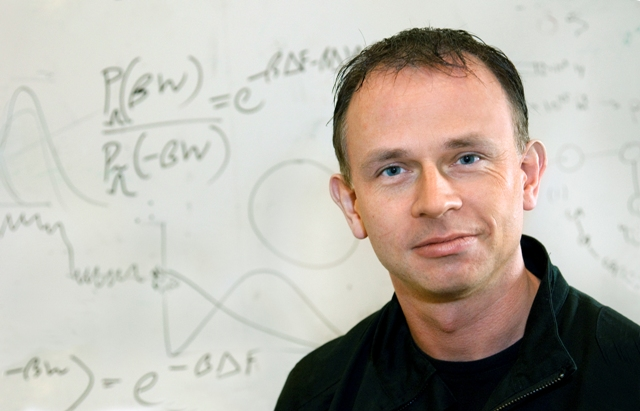
\includegraphics[width=.5\textwidth]{Gavin_Crooks.jpg}
            }
        \end{figure}
    \end{frame}
    \begin{frame}{正则系综与自由能}
        当系统与一个温度为$T$的大热库有热接触时, 平衡态系综的微观态分布满足, 
        \begin{equation}
            \rho(\vb*x) = \ee^{\beta(F - H(\vb*x))}, \quad \int_\Gamma\dd\vb*x\ \rho(\vb*x) = 1,\quad \beta = \frac1{k_B T}
        \end{equation}
        $F$为自由能, 由归一化决定,
        \begin{equation}
            \ee^{-\beta F} = \int_\Gamma\dd\vb*x\ \ee^{- \beta H(\vb*x)}
        \end{equation}
        更加普适的定义是,
        \begin{equation}
            F = \expval{H} - T S,\quad S = -\int_\Gamma\dd\vb*x\ \rho(\vb*x)\ln \rho(\vb*x)
        \end{equation}
    \end{frame}
    \begin{frame}{热力学第二定律}
        \begin{columns}
            \column{.5\textwidth}
            热力学第二定律,
            \begin{equation}
                \dbar Q \leqslant T\dd S 
            \end{equation}
            当系统和大热库始终处于热平衡的情况下, 从$A\to B$,
            \begin{equation}
                F_B - F_A = \Delta F \leqslant W^F 
            \end{equation}
            统计解释,
            \begin{equation}
                \Delta F \leqslant \expval{W^F} = \int W\rho^F(W)\dd W
            \end{equation}
            \column{.5\textwidth}
            \begin{figure}
                \centering
                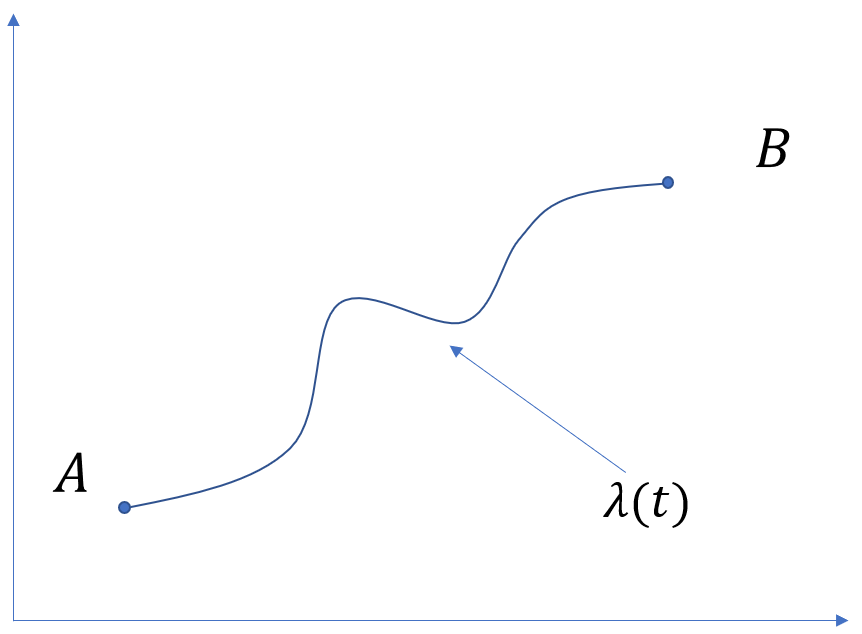
\includegraphics[width=\textwidth]{para.png}
                \caption{哈密顿量参数空间}
            \end{figure}
        \end{columns}
    \end{frame}
    \begin{frame}{热力学第二定理}
        \begin{columns}
            \column{.5\textwidth}
            我们考虑一下逆过程, $B\to A$,
            \begin{equation}
                F_A - F_B \leqslant \expval{W^R} = \int W\rho^R(W)\dd W
            \end{equation}
            把两个过程放在一起观察,
            \begin{equation}
                - \expval{W^R} \leqslant \Delta F \leqslant \expval{W^F}
            \end{equation}
            \pause
            \column{.5\textwidth}
            \begin{figure}
                \centering
                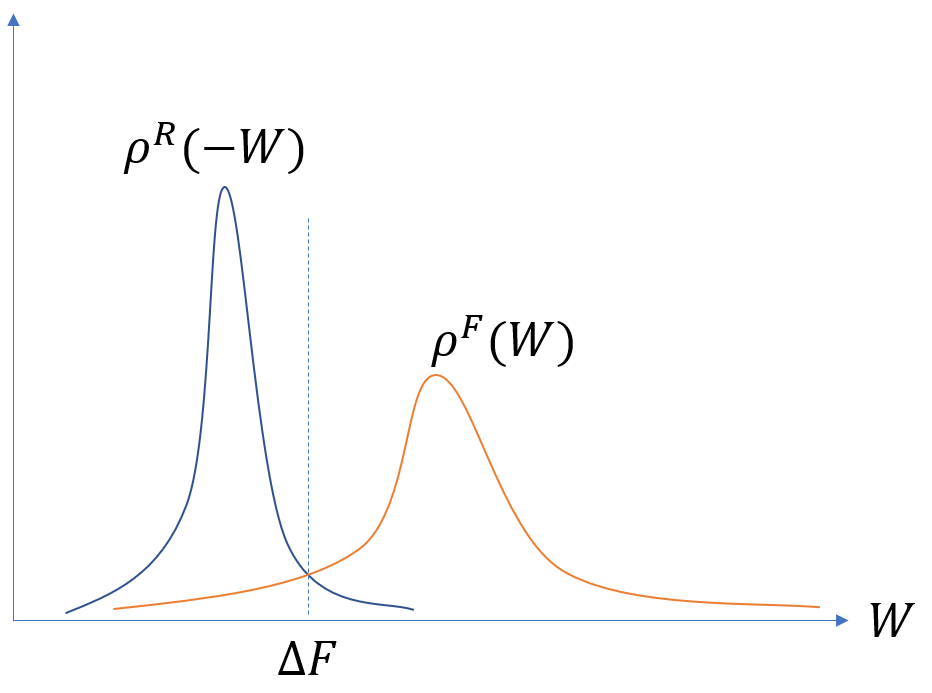
\includegraphics[width=\textwidth]{pw.png}
                \caption{概率分布}
            \end{figure}
        \end{columns}
    \end{frame}
    \begin{frame}{主要结论}
        \begin{itemize}
            \item Jarzynski Equality(JE):
            \begin{equation}
                \expval{\ee^{-\beta W}} = \ee^{-\beta \Delta F}
            \end{equation}
            \item Crooks Fluctuation Theorrem(CFT):
            \begin{equation}
                \frac{P^F(\omega)}{P^R(-\omega)} = \ee^{\omega}\quad\Rightarrow\quad \frac{\rho^F(W)}{\rho^R(-W)} = \ee^{\beta(W - \Delta F)}
            \end{equation}
        \end{itemize}
    \end{frame}
    %==========================================================
    \subsection{Jarzynski Equality(JE)}
    \begin{frame}{JE}
        \begin{alertblock}{Jarzynski Equality}
            将一个与温度为$T$的大热库热接触的系统, 改变系统的宏观参数, 从$A\to B$, $A$和$B$都是平衡态, 对于各种可能的做功, 我们有,
            \begin{equation}
                \expval{\ee^{-\beta W}} = \ee^{-\beta \Delta F}
            \end{equation}
        \end{alertblock}   
    \end{frame}
    \begin{frame}{证明}
        Jarzynski在1997年的PRL中实际上只给出了一种特殊情形下的证明, 我们考虑一个系统, 刚开始时和大热库处于热平衡, 满足正则系综, 然后进行控制参数的改变, 改变过程中和热库之间没有热量交换, 也无需处于平衡态, 结束之后, 保持控制参数不变, 系统和热库接触, 回到温度$T$. 
        
        哈密顿量$H = H(\vb*x,\lambda)$, 对于每一个参数$\lambda$, 都可以得到一个自由能$F_\lambda$,
        \begin{equation}
            \ee^{-\beta F_\lambda} = \int\dd\vb*x\ \ee^{-\beta H(\vb*x, \lambda)}
        \end{equation}
    \end{frame}
    \begin{frame}{证明}
        系统哈密顿量变化,
        \begin{equation}
            \dd H = \dd Q + \dd W \quad\Leftrightarrow\quad \dd{H(\vb*x(t),\lambda(t))} = \dd\vb*x\pdv{H}{\vb*x}  + \dd\lambda\pdv{H}{\lambda}
        \end{equation}
        可以知道做功$W$,
        \begin{equation}
            W = \int_0^{t_s} \dd t\ \dot\lambda\pdv{H}{\lambda} = H(\vb*x(t_s),B) - H(\vb*x(0),A)
        \end{equation}
        $W$与路径无关, $W = W(\vb*(x_0))$,
        \begin{equation}
            \expval{\ee^{-\beta W}} = \int \dd\vb*x(0)\ \frac{\ee^{-\beta H(\vb*x(0),A)}}{Z_A} \cdot \ee^{H(\vb*x(t_s),B) - H(\vb*x(0),A)} = \int  \dd\vb*x(0)\ \frac{\ee^{-\beta H(\vb*x_(t_s),B)}}{Z_A}
        \end{equation}
    \end{frame}
    \begin{frame}{证明}
        根据Liouville定理,
        \begin{equation*}
            \expval{\ee^{-\beta W}} = \int \dd\vb*x(t_s) \cdot \left|\pdv{\vb*x(t_s)}{\vb*x(0)}\right|^{-1} \cdot \frac{\ee^{-\beta H(\vb*x_(t_s),B)}}{Z_A} = \frac{Z_B}{Z_A}
        \end{equation*}
        \begin{equation}
            \Rightarrow\quad \expval{\ee^{-\beta W}} = \ee^{-\beta \Delta F}
        \end{equation}
    \end{frame}

    %==========================================================
    \subsection{Crooks Fluctuation Theorem(CFT)}
    \begin{frame}{系统演化}
        之前从哈密顿正则方程出发的演化方式, 相当于基于微正则系综. 这种方式的计算显然是有局限性的. 在之前的情形中, 若要考虑热量交换, 就必须考虑相互作用,
        \begin{equation}
            G(\vb*x,\vb*x') = H(\vb*x) + H'(\vb*x') + h_{int}(\vb*x,\vb*x')        
        \end{equation}
        事情变得非常复杂, 我们需要寻找新的角度来考察系统的演化.

        接下来的讨论中, 我们都假设哈密顿量应该是时间反演对称的(比如没有磁场).
    \end{frame}
    \begin{frame}{Markov Chain and Detailed Balance}
        \begin{block}{Markov Chain}
            有一列随机变量$\{X_0,X_1,X_2,\dots\}$, 若满足下式, 则称之为Markov链
            \begin{equation}
                \Pr(X_{n+1}=a_{n+1} | X_{n} = a_n, X_{n-1} = a_{n-1},\dots) = \Pr(X_{n+1}=a_{n+1} | X_{n} = a_n)
            \end{equation}
        \end{block}
        对于离散变量空间和离散时间的情形, 我们只需要知道每一步的转移矩阵$M_n$, 就知道系统的演化,
        \begin{equation}
            M_{n,ij} = \Pr(X_{n+1} = x_j| X_n = x_i),\ \sum_j M_{n,ij} = 1
        \end{equation}
        若$X_n$的概率分布是$\vb*\pi^{(n)} = [\pi^{(n)}_1,\pi^{(n)}_2,\dots]$,那么,
        \begin{equation}
            \vb*\pi^{(n+1)} = \vb*\pi^{(n)}M_n = \vb*\pi^{(0)}M_0\cdots M_{n-1}M_{n}
        \end{equation}
    \end{frame}
    \begin{frame}{Markov Chain and Detailed Balance}
        对于连续变量和连续时间的情形,
        \begin{equation}
            \rho(\vb*x, t) = \int p(\vb*x,t; \vb*x', t') \rho(\vb*x', t')\dd\vb*x', \quad \int p(\vb*x,t; \vb*x', t') \dd\vb*x = 1
        \end{equation}
        如果一个演化方式和初始时间无关, 只和时间差有关, 我们称这样的Markov链是时齐的(time homogeneous).
        \begin{equation}
            p(\vb*x,t; \vb*x',t') = p(\vb*x'\to\vb*x, \Delta t)
        \end{equation}
    \end{frame}
    \begin{frame}{Markov Chain and Detailed Balance}
        如果有一个分布在演化下保持不变, 这就是平衡态, 他应该满足,
        \begin{equation}
            \rho(\vb*x) = \int p(\vb*x'\to\vb*x, t)\rho(\vb*x')\dd\vb*x',\quad\forall t>0
        \end{equation}
        显然平衡态对于转移概率$p(\vb*x'\to\vb*x,t)$的约束在数学上并不那么强, 我们基于物理的考虑给他赋予一些新的性质.
        \begin{block}{Detailed Balance $\to$ Microscopically reversible}
            \noindent
            \begin{equation}
                \begin{split}
                    \rho(\vb*x)p(\vb*x\to\vb*x',t) &= \rho(\vb*x')p(\vb*x'\to\vb*x,t)\\ \Rightarrow
                    \rho(\hat{\vb*x})p(\hat{\vb*x}\to\hat{\vb*x}',t) &= \rho(\vb*x')p(\vb*x'\to\vb*x,t)\ \text{and}\ \rho(\vb*x) = \rho(\hat{\vb*x})                 
                \end{split}
            \end{equation}
            $\hat{\vb*x}$表示时间反演, i.e.$\ q\to q, p\to -p$.
        \end{block}
        % 时间反演对称性
        % \begin{equation}
        %     \rho(\hat{\vb*x}) = \rho(\vb*x)
        % \end{equation}
    \end{frame}
    \begin{frame}{Markov Chain and Detailed Balance}
        微观可逆性是平衡态的充分条件,
        \begin{equation}
            \int\dd\vb*x'\rho(\vb*x')p(\vb*x'\to\vb*x,t) = \int\dd\vb*x'\rho(\hat{\vb*x})p(\hat{\vb*x}\to\hat{\vb*x}',t) = \rho(\vb*x)
        \end{equation}
        对于不同的情况,
        \begin{table}[H]
            \centering
            \begin{tabular}{cccc}
                \toprule
                &微正则 & 正则 & 特殊($p$,$T$确定)\\
                \midrule
                $\dfrac{p(\hat{\vb*x}\to\hat{\vb*x}',t)}{p(\vb*x'\to\vb*x,t)}$ & 1 &$\ee^{-\beta(H(\vb*x') - H(\vb*x))}$ & $\ee^{-\beta(\Delta H + p \Delta V)}$\\
                \bottomrule
            \end{tabular}
        \end{table}
    \end{frame}
    \begin{frame}{概率密度}
        最后介绍一个求概率密度的公式, 现在有一个变量$x$的概率分布为$f(x)$, 对于一个新的变量$\omega = \omega(x)$, 它满足概率分布$\rho(\omega)$, 
        \begin{equation}
            \rho(\omega) = \int \delta(\omega(x) - \omega) f(x)\dd x
        \end{equation}
    \end{frame}
    \begin{frame}{CFT}
        \begin{alertblock}{Crooks Fluctuation Theorem}
            \begin{equation}
                \frac{P^F(\omega)}{P^R(-\omega)} = \ee^{\omega}
            \end{equation}
            系统和温度为$T$的大热库接触, $\omega$是一个确定参数变化过程$\lambda(t))(t\in[0,\tau])$中整个体系的熵产生, $P^F,P^R$是正过程和逆过程的熵产生分布函数.
        \end{alertblock}
        接下来都取, $k_B = 1$
    \end{frame}
    \begin{frame}{证明}
        对于相空间中某一条路径$\vb*x(t)$, 我们考虑沿这条路径的概率,
        $$
        F: x(0)\xrightarrow{\lambda(t_1)}x(t_1)\xrightarrow{\lambda(t_2)}x(t_2)\cdots \xrightarrow{\lambda(\tau)}x(\tau)
        $$
        $$
        R:  \hat x(0)\xleftarrow{\lambda(t_1)}\hat x(t_1)\xleftarrow{\lambda(t_2)}\hat x(t_2)\cdots \xleftarrow{\lambda(\tau)}\hat x(\tau)
        $$
        \begin{equation}
            \begin{split}
                \mathcal{P}^F[\vb*x(t)]\mathcal D[\vb*x(t)] &\approx\rho^F_0(\vb*x_0) \dd \vb*x_0p_1(\vb*x_0\to\vb*x_1,t_1)\dd\vb*x_1 \cdots p_n(\vb*x_{n-1}\to\vb*x_\tau,\tau-t_{n-1})\dd\vb*x_\tau\\
                \mathcal{P}^R[\hat{\vb*x}(\tau-t)]\mathcal D[\vb*x(t)] &\approx \dd\vb*x_0p_1(\hat{\vb*x}_0\leftarrow\hat{\vb*x}_1,t_1)\dd\vb*x_1 \cdots p_n(\hat{\vb*x}_{n-1}\leftarrow\hat{\vb*x}_\tau,\tau-t_{n-1})\dd\vb*x_\tau\rho^R_\tau(\hat{\vb*x}_\tau)
            \end{split}
        \end{equation}
        $p_i$表示在$\lambda(t_i)$的条件下进行演化. 利用之前的对于细致平衡的讨论,
        \[\dfrac{p(\hat{\vb*x}\to\hat{\vb*x}',t)}{p(\vb*x'\to\vb*x,t)} = \ee^{-\beta(H(\vb*x') - H(\hat{\vb*x}))}
            \]
    \end{frame}
    \begin{frame}{证明}
        可以得到微观可逆性条件,
        \begin{equation}
            \begin{split}
                \frac{\mathcal{P}^F[\vb*x(t)]}{\mathcal{P}^R[\hat{\vb*x}(\tau-t)]} &= \frac{\rho^F_0(\vb*x_0)}{\rho^R_\tau(\hat{\vb*x}_\tau)}\exp(-\beta\sum_i [H(\vb*x_i,\lambda_i) - H(\vb*x_{i-1},\lambda_i)]) \\
                &= \frac{\rho^F_0(\vb*x_0)}{\rho^R_\tau(\hat{\vb*x}_\tau)}\exp(-\beta\int\dd t\ \dot{\vb*x}\pdv{H(\vb*x,\lambda)}{\vb*x})\\
                &= \frac{\rho^F_0(\vb*x_0)}{\rho^R_\tau(\hat{\vb*x}_\tau)}\exp(-\beta Q)
            \end{split}
        \end{equation}
    \end{frame}
    \begin{frame}{证明}
        我们认为$S = \sum_{\vb*x} - \rho(\vb*x)\ln\rho(\vb*x)$, 
        正向熵产生$\omega^F$, 
        \begin{equation}
            \omega^F = \ln\rho^F_0(\vb*x(0)) - \ln\rho^F_\tau(\vb*x(\tau)) - \beta Q
        \end{equation}
        从而,
        \begin{equation}
            \ee^{\omega^F} = \frac{\rho^R_\tau(\hat{\vb*x}(\tau))}{\rho^F_\tau(\vb*x(\tau))}\cdot\frac{\mathcal{P}^F[\vb*x(t)]}{\mathcal{P}^R[\hat{\vb*x}(\tau-t)]} = \frac{\mathcal{P}^F[\vb*x(t)]}{\mathcal{P}^R[\hat{\vb*x}(\tau-t)]}
        \end{equation}
        最后一个等号我们假设有一个时间反演对称性,
        \begin{equation}
            \rho^F(\vb*x) = \rho^R(\hat{\vb*x})
        \end{equation}
        也可以得到$\omega^R = -\omega^F$
    \end{frame}
    \begin{frame}{证明}
        至此, 我们可以求出$P^F(\omega)$,
        \begin{equation}
            \begin{split}
                P^F(\omega) &= \int\delta(\omega-\omega^F) \mathcal P^F[\vb*x(t)]\mathcal D[\vb*x(t)]\\
                &= \ee^{\omega}\int\delta(\omega+\omega^R)\mathcal{P}^R[\hat{\vb*x}(\tau-t)]\mathcal D[\vb*x(t)]\\
                &= \ee^{\omega}P^R(-\omega)
            \end{split}
        \end{equation}
    \end{frame}
    \begin{frame}{CFT$\to$JE}
        对于初末态是正则系综平衡态的情形,
        \begin{equation}
            \rho^F_0(\vb*x) = \ee^{\beta(F_A - H(\vb*x,A))},\quad \rho^F_\tau(\vb*x) = \ee^{\beta(F_B - H(\vb*x,B))}
        \end{equation}
        从而, 熵产生为,
        \begin{equation}
            \begin{split}
                \omega^F &= \ln\rho^F_0(\vb*x(0)) - \ln\rho^F_\tau(\vb*x(\tau)) - \beta Q \\
                &=\beta(H(\vb*x(0),B) - H(\vb*x(\tau),A)-Q) - \beta(F_B-F_A) \\
                &= \beta(W-\Delta F)              
            \end{split}
        \end{equation}
        因此可以知道,
        \begin{equation}
            \frac{P^F(\omega)}{P^R(-\omega)} = \ee^{\omega}\quad\Rightarrow\quad \frac{\rho^F(W)}{\rho^R(-W)} = \ee^{\beta(W - \Delta F)}
        \end{equation}
    \end{frame}
    \begin{frame}{CFT$\to$JE}
        \begin{equation}
            \expval{\ee^{\beta( - W + \Delta F)}}_F = \int\dd W\rho^F(W) \ee^{\beta( - W + \Delta F)} = \int\dd W\rho^R(-W) = 1
        \end{equation}
        \pause
        
\includegraphics[width=100pt]{doggy.png}
    \end{frame}
    %==========================================================    
    \subsection{The Second Law of Thermodynamics}
    \begin{frame}{热力学第二定律}
        热力学第二定理统计解释, 
        \begin{equation}
            \expval{\ee^{-\omega}} = \int\dd \omega P^F(\omega) \ee^{-\omega} = \int\dd \omega P^R(-\omega) = 1
        \end{equation}
        利用Jensen不等式,
        \begin{equation}
            1 = \expval{\ee^{-\omega}} \geqslant \ee^{-\expval{\omega}}\quad\Rightarrow\quad \expval{\omega} \geqslant 0
        \end{equation}
    \end{frame}


%++++++++++++++++++++++++++++++++++++++++++++++++++++++++++++++++++++++++++++++++++++++++++++++++++++++++++++++++++++++++++++++++++++++++++++++++++++++++++++++++++++++++++++++++++++++++++++++++++++++++++++++++++++++++++++++++++++++++++++++++++++++++++
\section{Experiment}
    \subsection{JE}
    \begin{frame}{体系选择}
        我们需要验证JE, 利用数学上的相关公式,
        \begin{equation}
            \Delta F = -\frac1\beta \ln \expval{\ee^{-\beta W}} 
            = -\frac1\beta \sum_{n=1}^\infty \frac{(-\beta)^n}{n!} \kappa_n 
            \approx \expval{W} - \frac12\beta\sigma^2
        \end{equation}
        我们发现, 当$\sigma\beta$较大时, $\Delta F$会很大程度上取决于$W$取偏离$\expval{W}$较大的值, 从式子上看, 令$U = \ee^{-\beta W}$,
        \begin{equation}
            \rho_U(U) = \rho_W(W(U)) \left|\dv{W}{U}\right| = \rho_W(-\frac1\beta\ln U) \frac1{\beta U}
        \end{equation}
    \end{frame}
    \begin{frame}{gif}
        \begin{figure}[H]
            \centering
            \animategraphics[width=.8\textwidth]{10}{gif/anim}{0}{39}
            \caption{概率分布的偏离}
        \end{figure}
    \end{frame}
    \begin{frame}{体系选择}
        \begin{columns}
            \column{.7\textwidth}
            我们必须要选择一个介观的体系, 使得$\sigma\beta$不至于太大, 导致实验上误差太大. 
            \pause
            \begin{center}
                {\Large 展开\&折叠RNA!}
            \end{center}
            \column{.3\textwidth}
            \begin{figure}
                \centering
                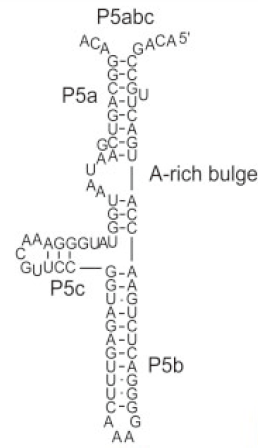
\includegraphics[width=.8\textwidth]{rna1.png}
                \caption{RNA}
            \end{figure}
        \end{columns}
    \end{frame}
    \begin{frame}{实验对系综的逼近}
        \begin{equation}
                \expval{\ee^{-\beta W}} = \lim_{N\to\infty} \expval{\ee^{-\beta W}}_N 
        \end{equation}
        三种对自由能的估计,
        \begin{equation}
            \begin{split}
                \text{Average work: } & W_A = \expval{W}_N\\
                \text{Fluctuation-dissipation estimate: } & W_{FD} = \expval{W}_N - \frac12\beta\sigma^2\\
                \text{Jarzynski equality: } & W_{JE} = \expval{\ee^{-\beta W}}_N
            \end{split}
        \end{equation}
    \end{frame}
    \begin{frame}{实验设计}
            \begin{figure}
                \centering
                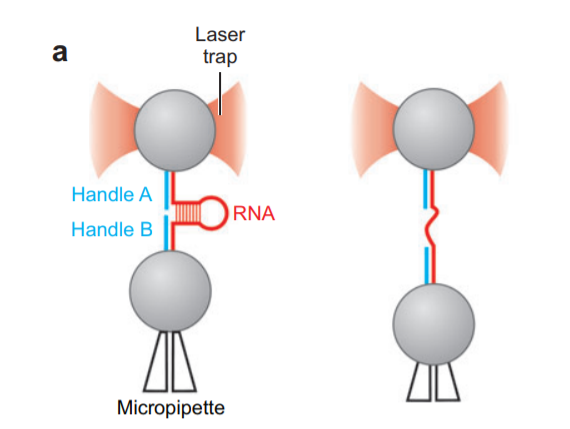
\includegraphics[width=.6\textwidth]{exp2.png}
                \caption{实验设计}
            \end{figure}
    \end{frame}
    \begin{frame}{光镊}
        \begin{figure}
            \centering
            \subfigure[]{
                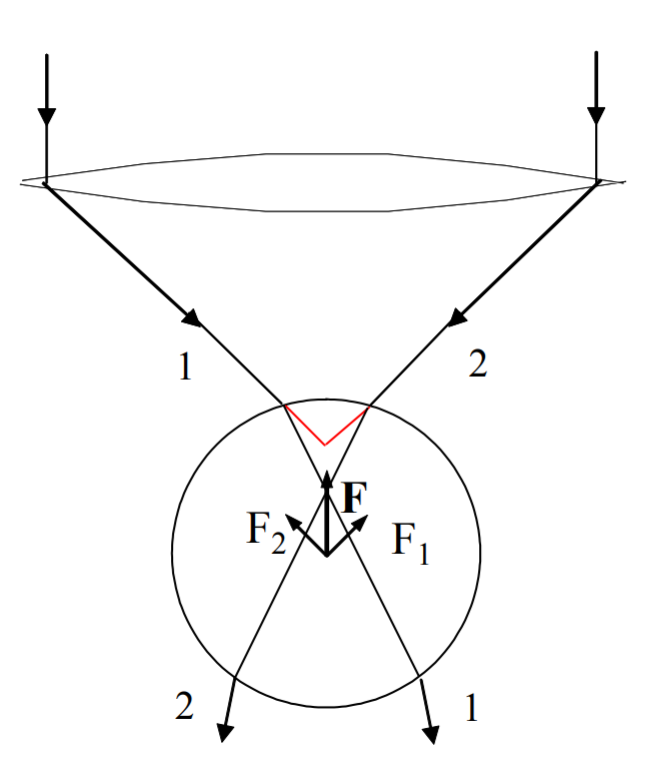
\includegraphics[height=.4\textwidth]{trap0.png}
            }
            \subfigure[]{
                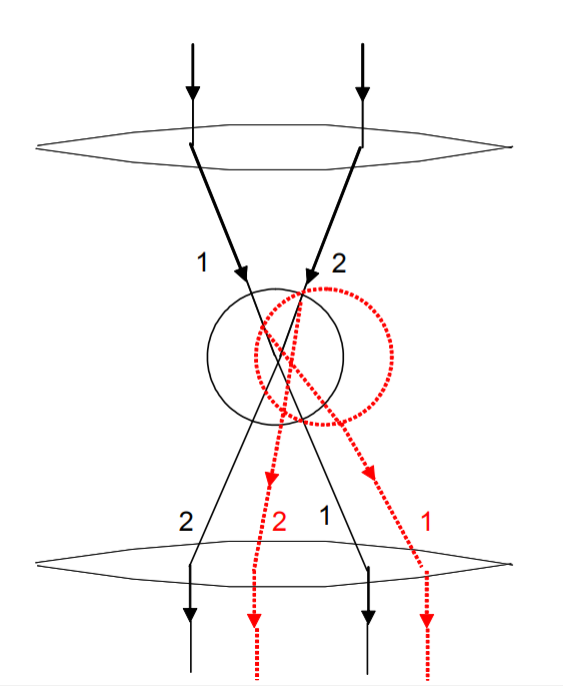
\includegraphics[height=.4\textwidth]{trap1.png}
            }
            \caption{光镊}
        \end{figure}
    \end{frame}
    \begin{frame}{实验结果}
        \begin{figure}
            \centering
            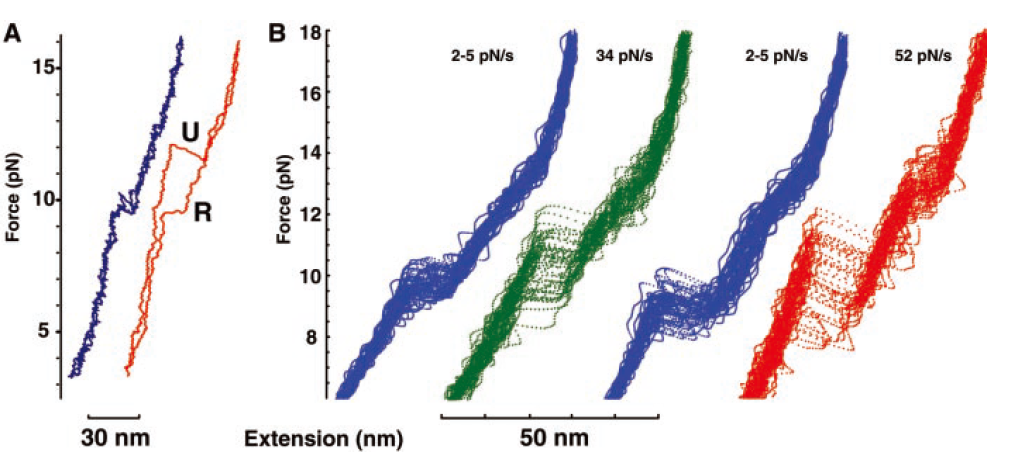
\includegraphics[height=.4\textwidth]{JE0.png}
            \caption{F-z曲线}
        \end{figure}
    \end{frame}
    \begin{frame}{实验结果}
        \begin{figure}
            \centering
            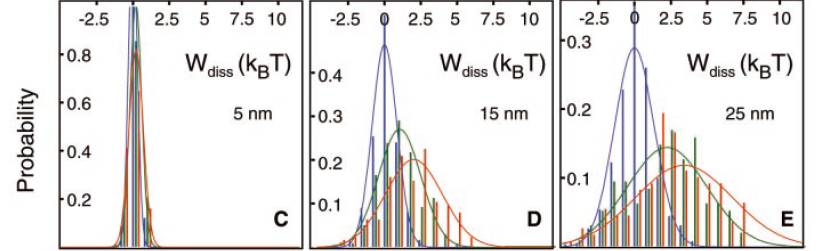
\includegraphics[height=.25\textwidth]{JE3.png}
            \caption{$W_{\text{diss}} = W - \Delta F$分布}
        \end{figure}
    \end{frame}
    \begin{frame}{实验结果}
        \begin{figure}
            \centering
            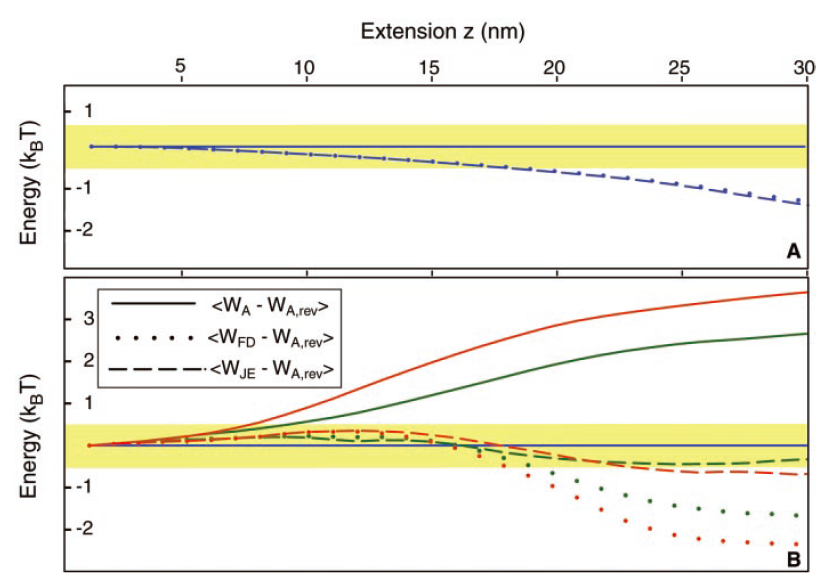
\includegraphics[height=.4\textwidth]{JE2.png}
            \caption{三种估计的对比}
        \end{figure}
    \end{frame}
    \subsection{CFT}
    \begin{frame}{CFT的实验验证}
        \begin{figure}
            \centering
            \subfigure[]{
                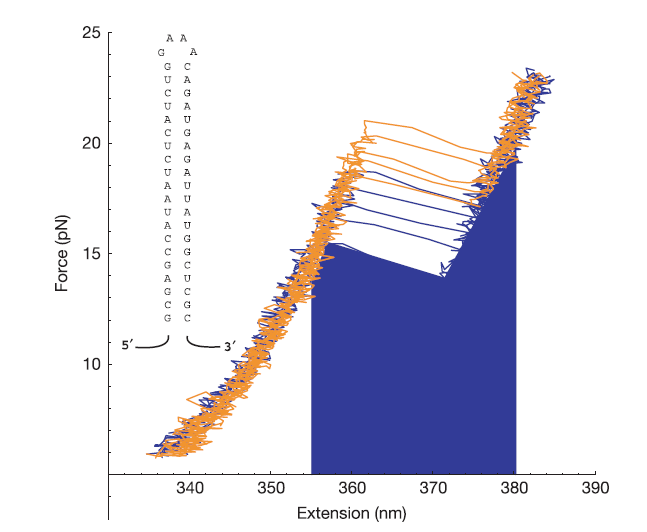
\includegraphics[height=.35\textwidth]{CFT0.png}
            }
            \subfigure[]{
                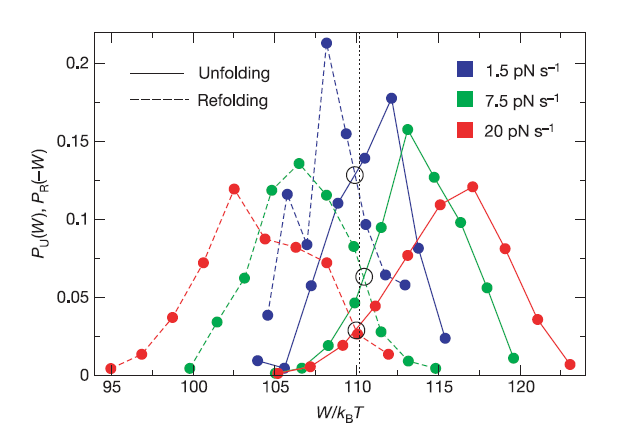
\includegraphics[height=.35\textwidth]{CFT1.png}
            }
        \end{figure}
    \end{frame}
    \begin{frame}{CFT的实验验证}
        \begin{figure}
            \centering
            \subfigure[非Gauss分布]{
                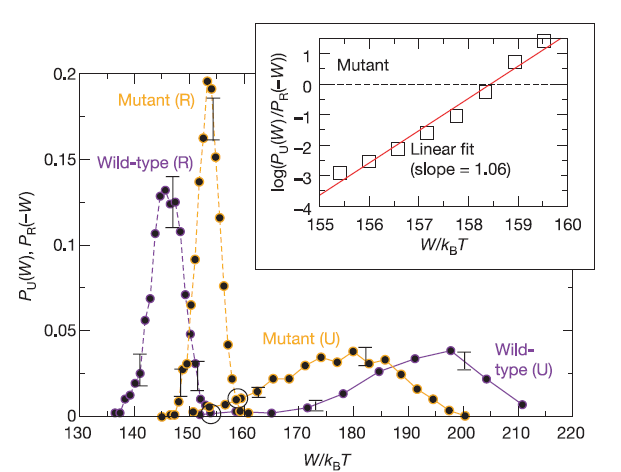
\includegraphics[height=.35\textwidth]{CFT2.png}
            }
            \subfigure[与BAR方法(数值模拟)对比]{
                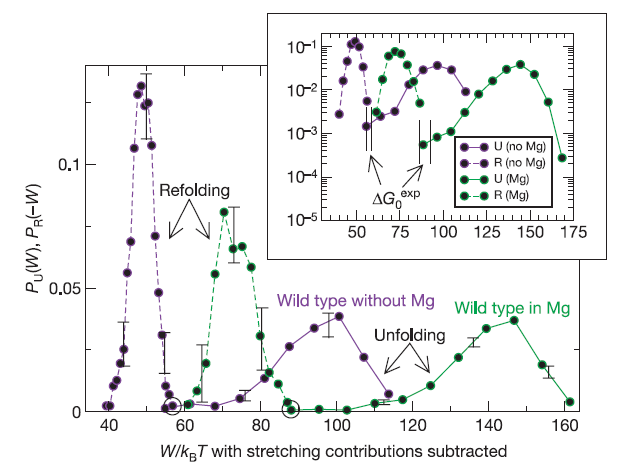
\includegraphics[height=.35\textwidth]{CFT3.png}
            }
        \end{figure}
    \end{frame}
% \end{document}
    
    % \section{Jarzynski等式}
    %     \subsection{发展过程}
    %     \subsection{等式证明}
%     \begin{frame}{Jarzynski等式}
%         \begin{columns}
%             \column{.7\textwidth}
%             \begin{alertblock}{Jarzynski等式}
%                 对于一个和大热库(温度为$T$)有热交换的系统, 从一个平衡态$A$出发, 由外界改变系统的某些宏观参数, 从而使得系统经历一个演化过程, 最后到达一个新的平衡态$B$, 对于系统的自由能$F$, 和过程中的做功$W$满足,
%                 \begin{equation}
%                     \exp (- \frac{\Delta F}{k_B T}) = \expval{\exp (- \frac{W}{k_B T})},\quad \Delta F = F_B - F_A
%                 \end{equation}
%                 其中, $\expval{\cdot}$表示对于初始状态$A$的正则系综取平均.
%             \end{alertblock}
%             \column{.3\textwidth}
%             \begin{figure}[H]
%                 \centering
%                 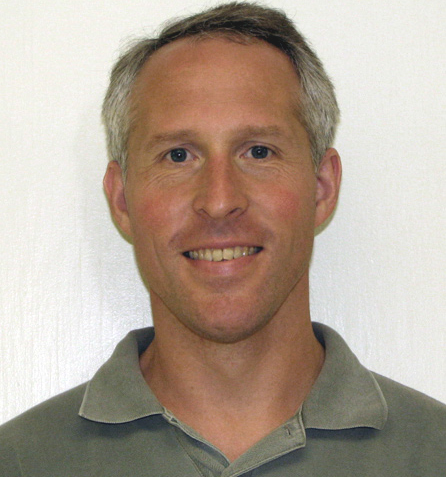
\includegraphics[width=.9\textwidth]{jarz.jpg}
%                 \caption{Christopher Jarzynski}
%             \end{figure}
%         \end{columns}
%     \end{frame}
%     \begin{frame}{详细解释}
%         \begin{columns}
%             \column{.6\textwidth}
%             \begin{itemize}
%                 \item 外界改变宏观参数, 但演化仍然满足正则方程, $H_\lambda(\vb*q,\vb*p)$
%                 \item 参数改变的路径是确定的, 关于时间的函数关系不受限制, $\gamma$
%                 \item 过程中可以是非平衡态, 但是初末态是平衡态, 且温度相同
%             \end{itemize}
%             \column{.4\textwidth}
%             \begin{figure}[H
%                 ]
%                 \centering
%                 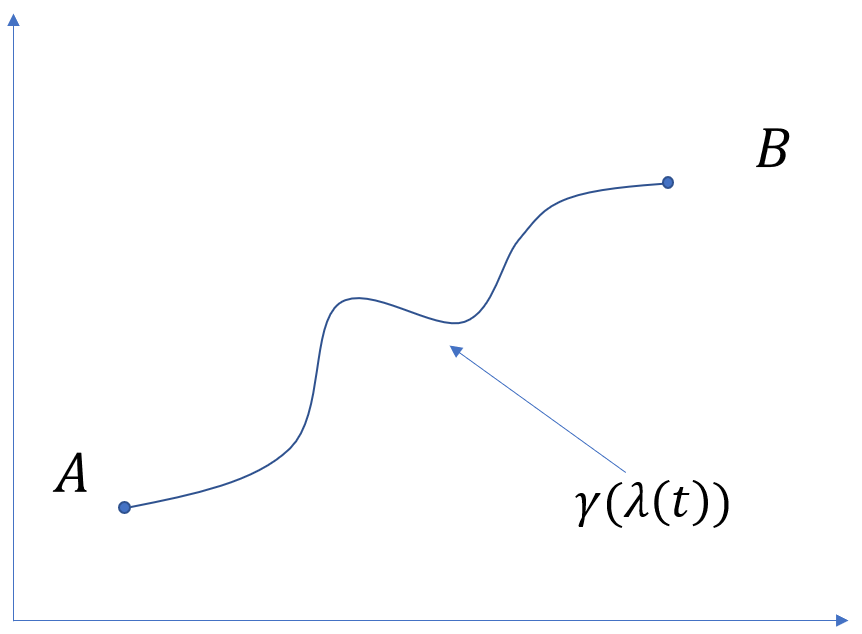
\includegraphics[width=\textwidth]{parameter.png}
%                 \caption{参数空间变化}
%             \end{figure}
%         \end{columns}
%     \end{frame}
%     \begin{frame}{证明}
%         我们先考虑孤立系统的情况, 假设曲线参数$\lambda\in[0,1]$, 哈密顿量为$H_\lambda(\vb*x)$, 外界对系统做功,
%         \begin{equation}
%             W = \int_0^{t_s} \dd t \dot\lambda \pdv{H_\lambda(\vb*x(t))}{\lambda}
%         \end{equation}
%         极限情形, $\dot\lambda \to \infty, t_s\to 0$, 这样系统参数瞬时变化, 
%         \begin{gather*}
%             W = \int_0^1 \dd\lambda\pdv{H_\lambda(\vb*x(0))}{\lambda} = H_1(\vb*x(0)) - H_0(\vb*x(0)) \\
%             \expval{\ee^{-\beta W}} = \int_\Gamma\dd\vb*x_0 \dfrac{\ee^{-\beta H_0(\vb*x_0)}}{Z_0} \cdot \ee^{-\beta (H_1(\vb*x_0) - H_0(\vb*x_0))} = \frac{Z_1}{Z_0}
%         \end{gather*}
%     \end{frame}
%     \begin{frame}{证明\ --\ 极限情形}
%         极限情形, $\dot\lambda \to \infty, t_s\to 0$, 这样系统参数瞬时变化, 
%         \begin{gather*}
%             W = \int_0^1 \dd\lambda\pdv{H_\lambda(\vb*x(0))}{\lambda} = H_1(\vb*x(0)) - H_0(\vb*x(0)) \\
%             \expval{\ee^{-\beta W}} = \int_\Gamma\dd\vb*x_0 \dfrac{\ee^{-\beta H_0(\vb*x_0)}}{Z_0} \cdot \ee^{-\beta (H_1(\vb*x_0) - H_0(\vb*x_0))} = \frac{Z_1}{Z_0}
%         \end{gather*}
%         而若$\dot\lambda \to 0$, 系统准静态演化, 可逆过程所有的做功都等于$\Delta F$, 
%         $$
%         \expval{\ee^{-\beta \Delta F}} = \ee^{-\beta \Delta F}
%         $$
%     \end{frame}
%     \begin{frame}{证明\ --\ 一般情形}
%         变积分变量为$\lambda$, 那么应当有$t = t(\lambda), \vb*x(t) = \vb*x(t(\lambda))$
%         \begin{equation}
%             \begin{split}
%                 \dv{H_\lambda(\vb*x(t(\lambda)))}{\lambda} &= \pdv{H_\lambda}{\lambda} + \pdv{H_\lambda}{x_\alpha} \dot x_\alpha\cdot \frac1{\dot\lambda}\\
%                 &= \pdv{H_\lambda}{\lambda} + \omega_{\alpha\beta}\pdv{H_\lambda}{x_\alpha}\pdv{H_\lambda}{x_\beta}\\ 
%                 &= \pdv{H_\lambda}{\lambda}
%             \end{split}
%         \end{equation}
%         因此,
%         \begin{equation}
%             W = \int_0^1 \dd \lambda \dv{H_\lambda}{\lambda} = H_1(\vb*x(t_s)) - H_0(\vb*x(0))
%         \end{equation}
%     \end{frame}
%     \begin{frame}{证明}
%         再经过一段时间的弛豫, 到达平衡态, 此过程外界不做功, 微观自由度按照正则方程演化
%         $$H_1(\vb*x(t_f)) = H_1(\vb*x(t_s))$$
%         因此,
%         \begin{equation}
%             \begin{split}
%                 \expval{\ee^{-\beta W}} &= \int_\Gamma\dd\vb*x_0 \dfrac{\ee^{-\beta H_0(\vb*x_0)}}{Z_0} \cdot \ee^{-\beta (H_1(\vb*x_{t_f}) - H_0(\vb*x_0))}\\
%                 &= \int_\Gamma\dd\vb*x_0 \dfrac{\ee^{-\beta H_1(\vb*x_{t_f})}}{Z_0}
%             \end{split}
%         \end{equation}
%         由Liouville定理, $\dd\vb*x_t = \dd\vb*x_0$,
%         \begin{equation}
%             \expval{\ee^{-\beta W}} = \frac1{Z_0} \int_\Gamma \dd\vb*x\ \ee^{-\beta H_1(\vb*x)} = \frac{Z_1}{Z_0}
%         \end{equation}
%     \end{frame}
%     \begin{frame}{证明}
%         接下来, 我们来考虑有热库的情形, 整个系统的哈密顿量,
%         \begin{equation}
%             \mathscr{H}_\lambda(\vb*x,\vb*x') = H_\lambda(\vb*x) + H'(\vb*x') + h_{int} (\vb*x, \vb*x')
%         \end{equation}
%         把整个系统视作整体, 那么,
%         \begin{equation}
%             W = \mathscr H_1(\vb*y(t_f)) - \mathscr H_0(\vb*y(0)),\quad \vb*y = (\vb*x, \vb*x')
%         \end{equation}
%         按照孤立系统的结论,
%         \begin{equation}
%             \int_{\Gamma\times\Gamma'}\dd\vb*y_0 \frac{\ee^{-\beta\mathscr H_0}}{\mathscr Z_0} \cdot \ee^{-\beta W} = \frac{\mathscr Z_1}{\mathscr Z_0}
%         \end{equation}
%     \end{frame}
%     \begin{frame}{证明\ -- \ 对于相互作用项的近似}
        
%     \end{frame}
%     % \begin{frame}{gif page}
%     %     \begin{figure}[H]
%     %         \centering
%     %         \animategraphics[width=.8\textwidth]{10}{gif/anim}{0}{39}
%     %         \caption{变化}
%     %     \end{figure}
%     % \end{frame}
%     \subsection{实验}

% \section{涨落定理}
%     \subsection{Crooks Fluctuation Theorem(CFT)}
%     \subsection{Transient Fluctuation Theorem(TFT)}

%====================================================================================
\begin{frame}[allowframebreaks]
    \nocite{*}
	\frametitle{References}
	\printbibliography[title={References}]
\end{frame}
\end{document}